\documentclass[
	10pt,								% globale Schriftgröße
	parskip=half-,						% setzt Absatzabstand hoch
	paper=a4,							% Format
	english,ngerman,					% lädt Sprachpakete
	]{scrartcl}							% Dokumentenklasse

% //////////////////// Pakete laden ////////////////////
\usepackage{amsmath}			% MUSS vor fontspec geladen werden
\usepackage{mathtools}			% modifiziert amsmath
\usepackage{amssymb}			% mathematische symbole, für \ceckmarks
\usepackage{amsthm}				% für proof
\usepackage{mathrsfs}			% für \mathscr
\usepackage{latexsym}
\usepackage{marvosym}				% für Lightning

\usepackage{fontspec} 			% funktioniert nur mit den neueren Compilern z.B. XeLaTeX
\usepackage{microtype}			% für bessere Worttrennung
\usepackage[ngerman]{babel} 	% Spracheinstellung
\usepackage{csquotes}
\usepackage{lmodern}			% verändert verwendete Schriftart, damit sie weniger pixelig ist

\usepackage{verbatim}
\usepackage{listings}			% Für Quellcode

\usepackage{graphicx}
\usepackage{tabularx}			% für Tabellen mit gleicher Spaltenbreite und automatischen Umbrüchen
\usepackage{fullpage}
\usepackage{multirow}			% für multirow in tabulars
\usepackage{rotate}
\usepackage[cmyk,table]{xcolor} % um Farben zu benutzen, kann mehr als das Paket color
\usepackage[					% Verlinkungen
	colorlinks,					% farbige Schrift, statt farbiger Rahmen
	linktocpage,				% verlinkt im Abb.Verzeichnis Seitenzahl statt Bildunterschrift
	linkcolor=blue				% setzt Farbe der Links auf blau
	]{hyperref}					% nur für digitale Anwendungen, url = "http://www.example.com"
\usepackage{url}				% für Webadressen wie e-mail usw.: "\url{http://www.example.com}"

\usepackage{enumerate}			% für versch. Aufzählungezeichen wie z.B. a)
\usepackage{xspace}				% folgt ein Leerzeichen nach einem \Befehl, wird es nicht verschluckt.
\usepackage{cancel}				% für das Durchstreichen u.a. in Matheformeln mit \cancel
\usepackage{float}              % zum Forcieren der Position von figure-Umgebungen

% zum Zeichnen (u.a. von Graphen)
\usepackage{fp}
\usepackage{tikz}
\usetikzlibrary{tikzmark}			% für \tikzmark{toRemember}
\usetikzlibrary{positioning}	% verbesserte Positionierung der Knoten
\usetikzlibrary{automata}		% für Automaten (GTI)
\usetikzlibrary{arrows}
\usetikzlibrary{shapes}
\usetikzlibrary{decorations.pathmorphing}
\usetikzlibrary{decorations.pathreplacing}
\usetikzlibrary{decorations.shapes}
\usetikzlibrary{decorations.text}

% //////////////////// Syntaxhighlighting ////////////////////
\lstloadlanguages{Python, Haskell, [LaTeX]TeX, Java}
\lstset{
   basicstyle=\footnotesize\ttfamily,	% \scriptsize the size of the fonts that are used for the code
   backgroundcolor = \color{bgcolour},	% legt Farbe der Box fest
   breakatwhitespace=false,	% sets if automatic breaks should only happen at whitespace
   breaklines=true,			% sets automatic line breaking
   captionpos=t,				% sets the caption-position to bottom, t for top
   commentstyle=\color{codeblue}\ttfamily,% comment style
   frame=single,				% adds a frame around the code
   keepspaces=true,			% keeps spaces in text, useful for keeping indentation
							% of code (possibly needs columns=flexible)
   keywordstyle=\bfseries\ttfamily\color{codepurple},% keyword style
   numbers=left,				% where to put the line-numbers;
   							% possible values are (none, left, right)
   numberstyle=\tiny\color{codegreen},	% the style that is used for the line-numbers
   numbersep=5pt,			% how far the line-numbers are from the code
   stepnumber=1,				% nummeriert nur jede i-te Zeile
   showspaces=false,			% show spaces everywhere adding particular underscores;
							% it overrides 'showstringspaces'
   showstringspaces=false,	% underline spaces within strings only
   showtabs=false,			% show tabs within strings adding particular underscores
   flexiblecolumns=false,
   tabsize=1,				% the step between two line-numbers. If 1: each line will be numbered
   stringstyle=\color{orange}\ttfamily,	% string literal style
   numberblanklines=false,				% leere Zeilen werden nicht mitnummeriert
   xleftmargin=1.2em,					% Abstand zum linken Layoutrand
   xrightmargin=0.4em,					% Abstand zum rechten Layoutrand
   aboveskip=2ex, 
}

\lstdefinestyle{py}{
   language=Python,
}
\lstdefinestyle{hs}{
   language=Haskell,
}
\lstdefinestyle{tex}{
	language=[LaTeX]TeX,
	escapeinside={\%*}{*)},     % if you want to add LaTeX within your code
	texcsstyle=*\bfseries\color{blue},% hervorhebung der tex-Schlüsselwörter
	morekeywords={*,$,\{,\},\[,\],lstinputlisting,includegraphics,
	rowcolor,columncolor,listoffigures,lstlistoflistings,
	subsection,subsubsection,textcolor,tableofcontents,colorbox,
	fcolorbox,definecolor,cellcolor,url,linktocpage,subtitle,
	subject,maketitle,usetikzlibrary,node,path,addbibresource,
	printbibliography},% if you want to add more keywords to the set
     numbers=none,
     numbersep=0pt,
     xleftmargin=0.4em,
}

\lstdefinestyle{java}{
	language=Java,
	extendedchars=true,		% lets you use non-ASCII characters;
   						% for 8-bits encodings only, does not work with UTF-8
}

\lstdefinelanguage[x64]{Assembler}     % add a "x64" dialect of Assembler
   [x86masm]{Assembler} % based on the "x86masm" dialect
   % with these extra keywords:
   {morekeywords={CDQE,CQO,CMPSQ,CMPXCHG16B,JRCXZ,LODSQ,MOVSXD, %
                  POPFQ,PUSHFQ,SCASQ,STOSQ,IRETQ,RDTSCP,SWAPGS, %
                  rax,rdx,rcx,rbx,rsi,rdi,rsp,rbp, %
                  r8,r8d,r8w,r8b,r9,r9d,r9w,r9b}
}					% for 8-bits encodings only, does not work with UTF-8

\lstdefinestyle{c}{
	language=c,
	extendedchars=true,		% for 8-bits encodings only, does not work with UTF-8
}

% //////////////////// eigene Kommandos ////////////////////
\newcommand\FU{Freie Universität Berlin\xspace}% benötigt package xspace
\newcommand\gdw{g.\,d.\,w.\xspace}
\newcommand\oBdA{o.\,B.\,d.\,A.\xspace}
\newcommand{\Eu}{\texteuro}
\newcommand\N{\mathbb{N}\xspace}
\newcommand\Q{\mathbb{Q}\xspace}
\newcommand\R{\mathbb{R}\xspace}
\newcommand\Z{\mathbb{Z}\xspace}
\newcommand\ohneNull{\ensuremath{\backslash\lbrace 0\rbrace}}% \{0}
\let\dhALT\dh	% Schreibt Befehl \dh in \dhALT um
\renewcommand\dh{d.\,h.\xspace}	%renew überschreibt command \dh
\newcommand\Bolt{\;\text{\LARGE\raisebox{-0.3em}{\Lightning}\normalsize}\xspace}% Blitz
\newcommand\zz{\ensuremath{\raisebox{+0.25ex}{Z}% zu zeigen
			\kern-0.4em\raisebox{-0.25ex}{Z}%
			\;\xspace}}
\newcommand{\from}{\ensuremath{\colon}}
\newcommand{\floor}[1]{\lfloor{#1}\rfloor}
\newcommand{\ceil}[1]{\lceil{#1}\rceil}
 \renewcommand{\L}{\ensuremath{\mathcal{L}}\xspace}
 \renewcommand{\P}{\ensuremath{\mathcal{P}}\xspace}
 \newcommand{\NL}{\ensuremath{\mathcal{N}\kern-0.2em\mathcal{L}}\xspace}
 \newcommand{\NP}{\ensuremath{\mathcal{NP}}\xspace}

% //////////////////// Mathefunktionen ////////////////////
\DeclareMathOperator{\Landau}{\mathcal{O}}
\DeclareMathOperator{\True}{True}
\DeclareMathOperator{\False}{False}

% //////////////////// eigene Theoreme ////////////////////
\newtheorem{theorem}{Satz}
\newtheorem{corollary}[theorem]{Folgerung}
\newtheorem{lemma}[theorem]{Lemma}
\newtheorem{observation}[theorem]{Beobachtung}
\newtheorem{definition}[theorem]{Definition}
\newtheorem{Literatur}[theorem]{Literatur}
% konfiguriert proof
\makeatletter
\newenvironment{Proof}[1][\proofname]{\par
  \pushQED{\qed}%
  \normalfont \topsep6\p@\@plus6\p@\relax
  \trivlist
  \item[\hskip\labelsep
%         \itshape
        \bfseries
    #1\@addpunct{.}]\ignorespaces
}{%
  \popQED\endtrivlist\@endpefalse
}
\makeatother

% //////////////////// eigene Farben ////////////////////
\let\definecolor=\xdefinecolor
\definecolor{FUgreen}{RGB}{153,204,0}
\definecolor{FUblue}{RGB}{0,51,102}

\definecolor{middlegray}{rgb}{0.5,0.5,0.5}
\definecolor{lightgray}{rgb}{0.8,0.8,0.8}
\definecolor{orange}{rgb}{0.8,0.3,0.3}
\definecolor{azur}{rgb}{0,0.7,1}
\definecolor{yac}{rgb}{0.6,0.6,0.1}
\definecolor{Pink}{rgb}{1,0,0.6}

\definecolor{bgcolour}{rgb}{0.97,0.97,0.97}
\definecolor{codegreen}{rgb}{0,0.6,0}
\definecolor{codegray}{rgb}{0.35,0.35,0.35}
\definecolor{codepurple}{rgb}{0.58,0,0.82}
\definecolor{codeblue}{rgb}{0.4,0.5,1}

% //////////////////// eigene Settings ////////////////////

\textheight = 230mm		% Höhe des Satzspiegels / Layouts
\footskip = 10ex			% Abstand zw. Fußzeile und Grundlinie letzter Textzeile
\parindent 0pt			% verhindert Einrückung der 1. Zeile eines Absatzes
\setkomafont{sectioning}{\rmfamily\bfseries}% setzt Ü-Schriften in Serifen, {disposition}
\graphicspath{ {./src/} } 
\usepackage{hyperref}

\newcommand{\dozent}{Volker Roth}
\newcommand{\tutor}{Oliver Wiese}
\newcommand{\tutoriumNo}{02\\Materialien: Latex, VSC, Skript}
\newcommand{\ubungNo}{07}
\newcommand{\veranstaltung}{Rechnersicherheit}
\newcommand{\semester}{SoSe 21}

% /////////////////////// BEGIN DOKUMENT /////////////////////////
\begin{document}
% /////////////////////// BEGIN TITLEPAGE /////////////////////////
\begin{titlepage}
	\subject{\dozent}
	\title{\veranstaltung, \semester}
	\subtitle{\Large Übung \ubungNo\\ \large\vspace{1ex} TutorIn: \tutor\\ Tutorium \tutoriumNo}
	\author{\studenten}
	\date{\normalsize \today}
\end{titlepage}

\maketitle								% Erstellt das Titelblatt
\vspace*{-10cm}							% rückt Logo an den oberen Seitenrand
\makebox[\dimexpr\textwidth+1cm][r]{	%rechtsbündig und geht rechts 1cm über Layout hinaus
	
\includegraphics[width=0.4\textwidth]{src/fu_logo} % fügt FU-Logo ein
}
% /////////////////////// END TITLEPAGE /////////////////////////

\vspace{7cm}							% Abstand
\rule{\linewidth}{0.8pt}				% horizontale Linie

% /////////////////////// Task 1 /////////////////////////
\section{Rainbow tables}
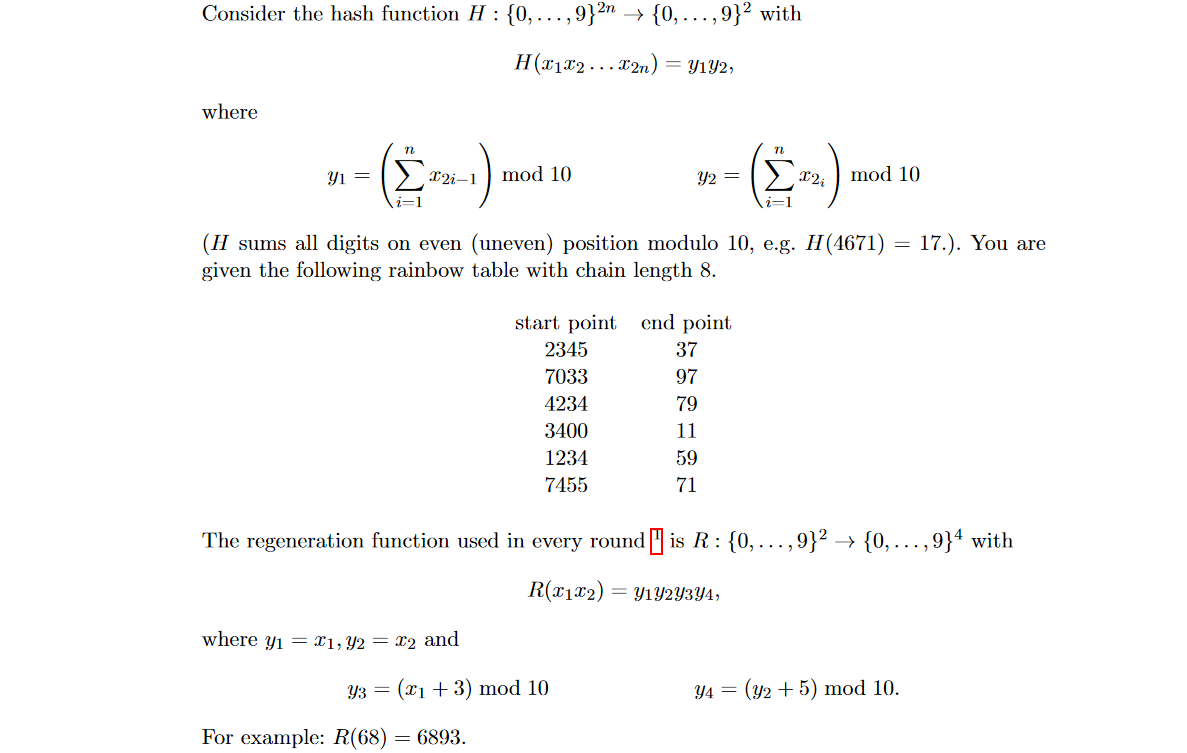
\includegraphics[width=\textwidth]{src/u7/task1.png}
\begin{enumerate}[(a)]

    % /////////////////////// a /////////////////////////
    \item {\itshape Find one inverse of the hash value 91 using the table above and document your steps.}
    \begin{itemize}
        \item We have two different approaches.
        \begin{enumerate}[1.]
            \item \textbf{Solution}: Finding the inverse of the hash value $h_1$ = 91, by using R and H on \underline{$h_1$}. 
                \begin{enumerate}[{1}.1]
                    \item Search for $h_1$ = 91 in the table (end point column) $\rightarrow$ not found.
                    \item Use the regeneration function R on $h_1$ $\rightarrow$ R(91) = 9126
                    \item Use the hash function H on the result $\rightarrow$ H(9126) = 17
                    \item (And now repeat these steps until found): 
                    \\ Search for $h_1$ = 17 in the table (end point column) $\rightarrow$ not found.
                    \item Use the regeneration function R on $h_1$ $\rightarrow$ R(17) = 1742
                    \item Use the hash function H on the result $\rightarrow$ H(1742) = 59
                    \item Search for $h_1$ = 59 in the table (end point column) $\rightarrow$ found entry!
                \end{enumerate}
                  
            \
            \item \textbf{Solution}: Finding the inverse of the hash value 91, by using R and H on \underline{every end point entry} of the hash table.
                \begin{enumerate}[{2}.1]
                
                    \item Search for 91 in the table (end point column) $\rightarrow$ not found.
                    \item Use the regeneration function R on every entry of that column:
                    \\{%\Large
                    \begin{tabular}{c c c}
                        \textbf{start point} & \textbf{\textcolor{blue}{R(\textcolor{green}{end point})}} & \textbf{\textcolor{green}{end point}} \\
                        2345 & 3672 & 37 \\
                        7033 & 9722 & 97 \\
                        4234 & 7904 & 79 \\
                        3400 & 1146 & 11 \\
                        1234 & 5984 & 59 \\
                        7455 & 7105 & 71 
                    \end{tabular}
                    } 
                    
                    \item Use the hash function H on every result:
                    \\{%\Large
                    \begin{tabular}{c c c c}
                        \textbf{start point} & \textbf{\textcolor{blue}{H(\textcolor{green}{R})}} & \textbf{\textcolor{green}{R}} & \textbf{end point} \\
                        2345 & 99 & 3672 & 37 \\
                        7033 & 19 & 9722 & 97 \\
                        4234 & 73 & 7904 & 79 \\
                        3400 & 57 & 1146 & 11 \\
                        1234 & 33 & 5984 & 59 \\
                        7455 & 76 & 7105 & 71 
                    \end{tabular}
                    } 
                    
                    
                    \item (And now repeat these steps until found): 
                    \\ Search for 91 in the table (newly calculated hash column) $\rightarrow$ not found.
                    \item Use the regeneration function R on every entry of that column:
                    \\{%\Large
                    \begin{tabular}{c c c c c}
                        \textbf{start point} & \textbf{\textcolor{blue}{R(\textcolor{green}{H})}} & \textbf{\textcolor{green}{H}} & \textbf{R} & \textbf{end point} \\
                        2345 & 9924 & 99 & 3672 & 37 \\
                        7033 & 1944 & 19 & 9722 & 97 \\
                        4234 & 7308 & 73 & 7904 & 79 \\
                        3400 & 5782 & 57 & 1146 & 11 \\
                        1234 & 3368 & 33 & 5984 & 59 \\
                        7455 & 7610 & 76 & 7105 & 71 
                    \end{tabular}
                    }
                    
                    \item Use the hash function H on every result:
                    \\{%\Large
                    \begin{tabular}{c c c c c c}
                        \textbf{start point} & \textbf{\textcolor{blue}{H(\textcolor{green}{R})}} & \textbf{\textcolor{green}{R}} & \textbf{H} & \textbf{R} & \textbf{end point} \\
                        2345 & 13 & 9924 & 99 & 3672 & 37 \\
                        7033 & 53 & 1944 & 19 & 9722 & 97 \\
                        4234 & 71 & 7308 & 73 & 7904 & 79 \\
                        3400 & 39 & 5782 & 57 & 1146 & 11 \\
                        1234 & 91 & 3368 & 33 & 5984 & 59 \\
                        7455 & 77 & 7610 & 76 & 7105 & 71 
                    \end{tabular}
                    }
                    \item Search for 91 in the table (newly calculated hash column) $\rightarrow$ entry found!
                    
                    
                \end{enumerate}
        \end{enumerate} 
    \end{itemize}
\end{enumerate}

% /////////////////////// Task 2 /////////////////////////
\section{Your project}
\begin{enumerate}[(a)]
    % /////////////////////// a /////////////////////////
    \item {\itshape Personal message: A user should be able to send a personal message to another user. We still have one global chat room.}
    \begin{itemize}
        \item For this we just added a 'Command Handler' on the Server side. Example of it working:
        
        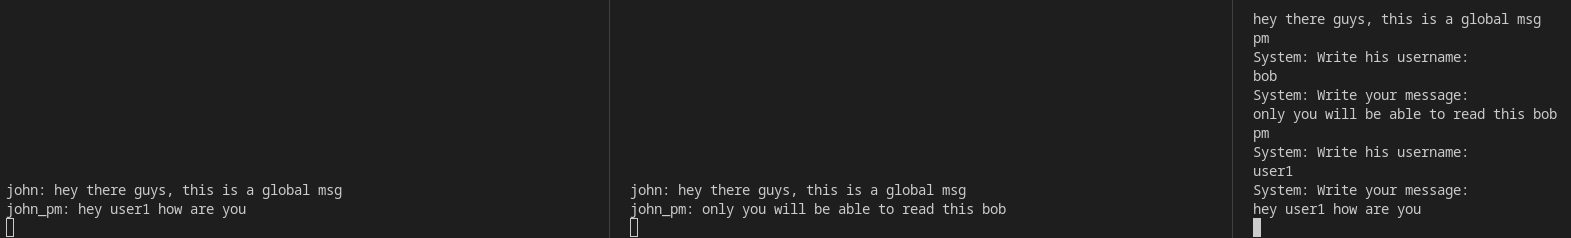
\includegraphics[width=\textwidth]{src/u7/1.png}
        
        \item Implementation:
        
        \lstinputlisting[language=python, linerange={18-35}, firstnumber = 18]{src/u7/commands_server.py}

    \end{itemize}
    
    
    % /////////////////////// b /////////////////////////
    \item {\itshape History: A user should have access to a communication history (for global chat and personal messages). The history has to be stored on the server side.}
    \begin{itemize}
        \item For this we added a 'log Handler' (history), which creates/write/returns log files of users and the global log file.
        We also added a new function in the 'Command Handler' on the server side. Example of it working:
        
        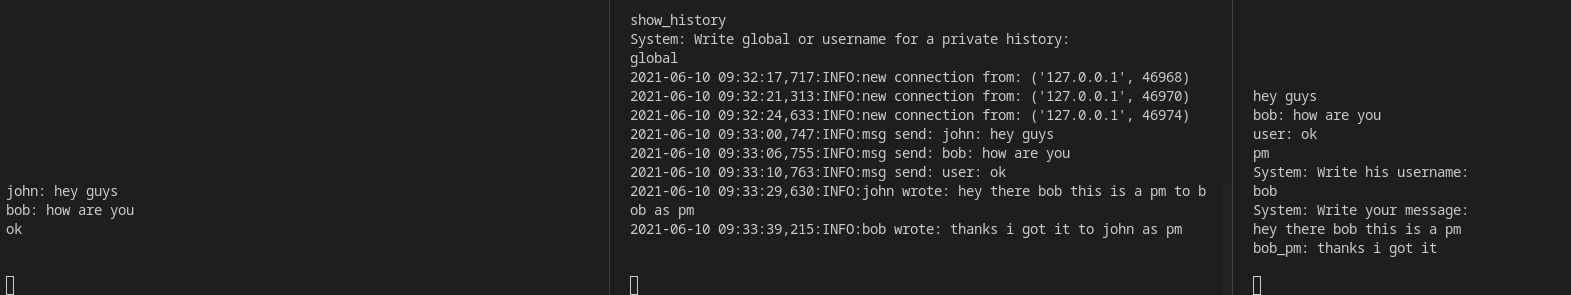
\includegraphics[width=\textwidth]{src/u7/2.png}
        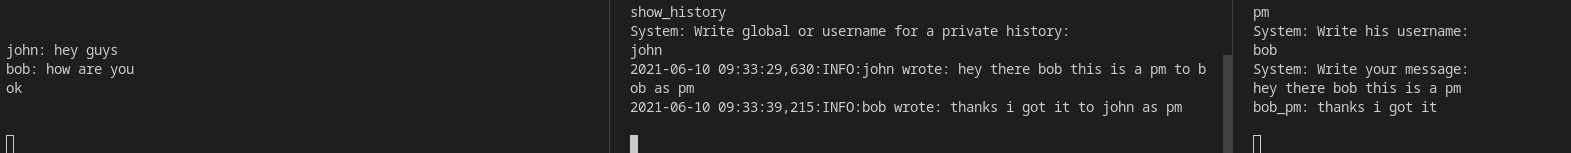
\includegraphics[width=\textwidth]{src/u7/3.png}

\newpage        
        \item Implementation:
        
        \lstinputlisting[language=python, linerange={37-46}, firstnumber = 37]{src/u7/commands_server.py}
        \lstinputlisting[language=python]{src/u7/log_handler.py}
    \end{itemize}Implementation

\newpage
    % /////////////////////// c /////////////////////////
    \item {\itshape Attachments: A user should be able to send files to other users and the chat room. Files should be stored on the server side (as part of the history) and client side (such that the user can open the file).}
    \begin{itemize}
        \item As for now the file is not saved on the client side. It will only print on his console. For this we added a 'Command Handler' on the client side. Example of it working:
        
        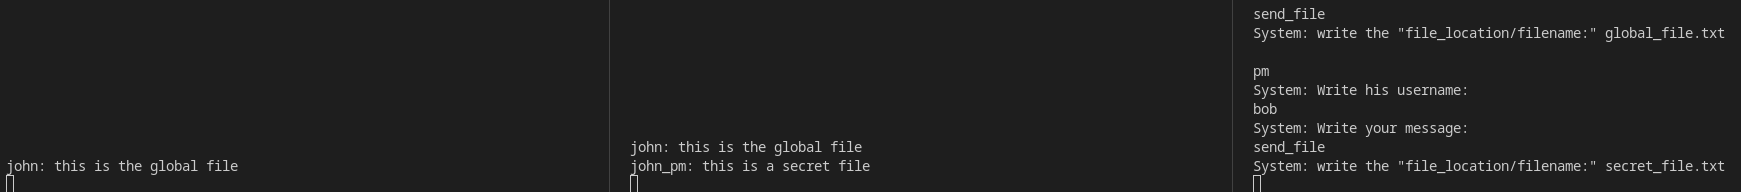
\includegraphics[width=\textwidth]{src/u7/4.png}
        
        \item Implementation:
        
        \lstinputlisting[language=python, linerange={15-19}, firstnumber = 15]{src/u7/commands_client.py}
    \end{itemize}

\end{enumerate}

\end{document}